\documentclass[xcolor=dvipsnames,table]{beamer}

\usepackage{latexsym}
\usepackage[utf8]{inputenc}
\usepackage[brazil]{babel}
\usepackage{amssymb}
\usepackage{amsmath}
\usepackage{stmaryrd}
\usepackage{fancybox}
\usepackage{datetime}
\usepackage[T1]{fontenc}
\usepackage{graphicx}
\usepackage{graphics}
\usepackage{url}
\usepackage{algorithmic}
\usepackage{algorithm}
\usepackage{acronym}
\usepackage{array}
\usepackage[normalem]{ulem}

\newtheorem{definicao}{Definio}
\newcommand{\tab}{\hspace*{2em}}

\mode<presentation>
{
  \definecolor{colortexto}{RGB}{0,0,0}
 
  \setbeamertemplate{background canvas}[vertical shading][ bottom=white!10,top=white!10]
  \setbeamercolor{normal text}{fg=colortexto} 

  \usetheme{Warsaw}
}

\title{Classe P} 

\author{
  Esdras Lins Bispo Jr. \\ \url{bispojr@ufg.br}
  } 
 \institute{
  Teoria da Computação \\Bacharelado em Ciência da Computação}
\date{\textbf{25 de julho de 2016} }

\logo{
\includegraphics[width=1cm]{images/ufgJataiLogo.png}}

\begin{document}

	\begin{frame}
		\titlepage
	\end{frame}

	\AtBeginSection{
		\begin{frame}{Sumário}%[allowframebreaks]{Sumário}
    		\tableofcontents[currentsection]
    		%\tableofcontents[currentsection, hideothersubsections]
		\end{frame}
	}

	\begin{frame}{Plano de Aula}
		\tableofcontents
		%\tableofcontents[hideallsubsections]
	\end{frame}
    
    \section{Pensamento}
	\begin{frame}{Pensamento}
  		\begin{center}
    		
\includegraphics[width=7cm]{images/pensamento.png}
  		\end{center}
	\end{frame}
	
	\begin{frame}{Pensamento}
		\begin{columns}
			\column{.4\textwidth}  		
		  		\begin{center}
		    		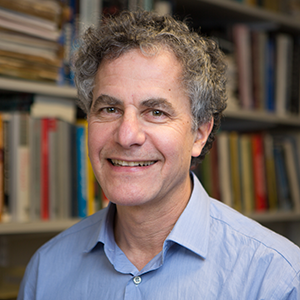
\includegraphics[height=.5\textheight]{images/sipser.png}
		  		\end{center}
			\column{.6\textwidth}  		
				\begin{block}{Frase}
					\begin{center}
						{\large Ignorar as árvores para ver a floresta não significa que uma é mais importante do que a outra.}
					\end{center}
				\end{block}		  		
		  		\begin{block}{Quem?}
		  			\begin{center}
						{\bf Michael Sipser (1954 -)} \\ Matemático e cientista da computação estadunidense.
					\end{center}
				\end{block}
		\end{columns}
	\end{frame}
	
%------------------------------------------

\section{Revisão}	
	\subsection{Classe P}
	\begin{frame}{Complexidade de Tempo}
		\begin{block}{Definição 7.7}
			Seja $t: \mathbb{N} \rightarrow \mathbb{R}^+$ uma função. Defina a {\bf classe de complexidade de tempo}, {\bf TIME($t(n)$)}, como sendo a coleção de todas as linguagens que são decidíveis por uma máquina de Turing de tempo $O(t(n))$.
		\end{block} 
		\begin{block}{Exemplo}
			\begin{itemize}
				\item $A = \{ 0^k 1^k$ | $k \geq 0 \}$
				\item $A \in$ {\bf TIME($n^2$)}, pois
				\item $M_1$ decide $A$ em tempo $O(n^2)$
			\end{itemize}
		\end{block}
	\end{frame}
	
	\begin{frame}[shrink]{Complexidade de Tempo}
		\begin{block}{Problema}
			Seja a linguagem $A = \{ 0^k 1^k$ | $k \geq 0 \}$. Quanto tempo uma máquina de Turing simples precisa para decidir $A$?
		\end{block} 
		\begin{block}{Descrição de uma possível MT simples}
			$M_1$ = ``Sobre a cadeia de entrada $\omega$:
			\begin{enumerate}
				\item Faça uma varredura na fita e {\it rejeite} se um 0 for encontrado à direita de um 1.
				\item Repita se ambos 0s e 1s permanecem sobre a fita:
				\begin{enumerate}
					\item Faça uma varredura na fita, cortando um único 0 e um único 1.
				\end{enumerate}
				\item Se 0s ainda permanecerem após todos os 1s tiverem sido cortados, ou se 1s ainda permanecerem após todos os 0s tiverem sido cortados, {\it rejeite}. Caso contrário, se nem 0s nem 1s permanecerem sobre a fita, {\it aceite}.
			\end{enumerate}
		\end{block}
	\end{frame}
	
	\begin{frame}{Complexidade de Tempo}
		\begin{block}{Problema}
			Existe uma máquina que decide assintoticamente \\a linguagem $A$ mais rapidamente?
		\end{block}
		\begin{block}{Com outras palavras...}
			$A \in$ {\bf TIME($t(n)$)}, para algum $t(n) = o(n^2)$?
		\end{block}
	\end{frame}
	
	\begin{frame}[shrink]{Complexidade de Tempo}
		\begin{block}{Descrição de uma outra MT simples}
			$M_2$ = ``Sobre a cadeia de entrada $\omega$:
			\begin{enumerate}
				\item Faça uma varredura na fita e {\it rejeite} se um 0 for encontrado à direita de um 1.
				\item Repita enquanto alguns 0s e alguns 1s permanecem sobre a fita:
				\begin{enumerate}
					\item Faça uma varredura na fita, verificando se o número total de 0s e 1s remanescentes é par ou ímpar. Se for ímpar, {\it rejeite}.
					\item Faça uma varredura novamente na fita, \\cortando alternadamente um 0 não e outro sim \\(começando com o primeiro 0) \\e então cortando alternadamente um 1 não e outro sim \\(começando com o primeiro 1).
				\end{enumerate}
				\item Se nenhum 0 e nenhum 1 permanecer sobre a fita, {\it aceite}. Caso contrário, {\it rejeite}.
			\end{enumerate}
		\end{block}
	\end{frame}
	
	\begin{frame}{Complexidade de Tempo}
		\begin{block}{Problema}
			Podemos decidir a linguagem $A$ em tempo $O(n)$ \\(também chamado {\bf tempo linear})?
		\end{block}
		\begin{exampleblock}{Sim... é possível!}
			Se utilizarmos uma máquina de Turing com duas fitas!
		\end{exampleblock}
	\end{frame}
	
	\begin{frame}[shrink]{Complexidade de Tempo}
		\begin{block}{Descrição de uma outra MT simples}
			$M_3$ = ``Sobre a cadeia de entrada $\omega$:
			\begin{enumerate}
				\item Faça uma varredura na fita e {\it rejeite} se um 0 for encontrado à direita de um 1.
				\item Faça uma varredura nos 0s sobre a fita 1 até o primeiro 1. \\Ao mesmo tempo, copie os 0s para a fita 2.
				\item Faça uma varredura nos 1s sobre a fita 1 até o final da entrada. Para cada 1 lido sobre a fita 1, corte um 0 sobre a fita 2. Se todos os 0s estiverem cortados antes que todos os 1s sejam lidos, {\it rejeite}.
				\item Se todos os 0s tiverem agora sido cortados, {\it aceite}. Se algum 0 permanecer, {\it rejeite}.
			\end{enumerate}
		\end{block}
	\end{frame}
	
	\subsection{Complexidade entre Modelos}	
	
	\begin{frame}{Relacionamentos de Complexidade entre Modelos}
		\begin{block}{Teorema 7.8}
			Seja $t(n)$ uma função, em que $t(n) \geq n$. Então toda máquina de Turing multifita de tempo $t(n)$ tem uma máquina de Turing de um única fita equivalente de tempo $O(t^2(n))$.
		\end{block}
		\begin{block}{Teorema 7.11}
			Seja $t(n)$ uma função, em que $t(n) \geq n$. Então toda máquina de Turing não-determinística de uma única fita de tempo $t(n)$ tem uma máquina de Turing de um única fita equivalente de tempo $2^{O(t(n))}$.	
		\end{block}
	\end{frame}
	
	\begin{frame}{A Classe P}
		\begin{block}{Diferenças de complexidade de tempo}
			\begin{itemize}
				\item MT simples $x$ MT multi-fita: \\potência quadrática (ou {\it polinomial})
				\item MT simples $x$ MT não-determinística: \\no máximo {\it exponencial}.
			\end{itemize} 		
		\end{block}
	\end{frame}
	
	\begin{frame}{A Classe P}
		\begin{block}{Diferenças entre as taxas de crescimento}
			{\bf Exemplo:} $n^3$ e $2^n$
			\begin{itemize}
				\item Admita $n = 1000$;
				\item Logo, $n^3 = 1$ bilhão;
				\item Mas, $2^n$ é maior que o número de átomos do universo.
			\end{itemize}
		\end{block}
	\end{frame}
	
	\begin{frame}{A Classe P}
		\begin{block}{Definição 7.12}
			{\bf P} é a classe de linguagens que são decidíveis em tempo polinomial sobre uma máquina de Turing determinística de uma única fita. \\Em outras palavras
			\begin{center}
				{\bf P} = $\bigcup\limits_{k}$ {\bf TIME ($n^k$)}.
			\end{center}
		\end{block}
		\begin{block}{{\bf P} é importante porque...}
			\begin{itemize} 
				\item {\bf P} é invariante para todos os modelos de computação polinomialmente equivalentes à máquina de Turing determinística de uma única fita;
				\item {\bf P} corresponde aproximadamente à classe de problemas que são realisticamente solúveis em um computador.
			\end{itemize}
		\end{block}
	\end{frame}
	
	\section{Classe P}
	
	\begin{frame}{A Classe P}
		\begin{block}{Problema do caminho em um grafo}
			$CAM = \{ \langle G, s, t \rangle \mbox{ | } G$ é um grafo direcionado que tem um caminho direcionado de $s$ para $t \}$.
		\end{block} \pause
		\begin{center}
			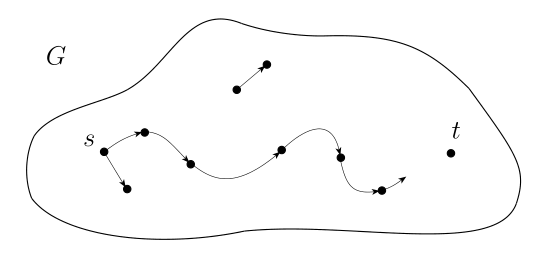
\includegraphics[width=8cm]{images/cam.png}
		\end{center}
	\end{frame}
	
	\begin{frame}{A Classe P}
		\begin{block}{Teorema 7.14}
			$CAM \in$ {\bf P}
		\end{block} \pause
		\begin{block}{Prova}
			$M$ = ``Sobre a cadeia de entrada $\langle G, s, t \rangle$ em que $G$ é um grafo direcionado com nós $s$ e $t$:
			\begin{enumerate}
				\item Ponha uma marca sobre o nó $s$.
				\item Repita o seguinte até que nenhum nó adicional seja marcado:
				\begin{enumerate}
					\item Faça uma varredura em todas as arestas de $G$. Se uma aresta $(a,b)$ for encontrada indo de um nó marcado $a$ para um nó não marcado $b$, marque o nó $b$.
				\end{enumerate}
				\item Se $t$ estiver marcado, {\it aceite}. Caso contrário, {\it rejeite}.
			\end{enumerate}
		\end{block}
	\end{frame}
	
	\begin{frame}{A Classe P}
		\begin{block}{Problema dos números primos entre si}
			PRIM-ES $= \{ \langle x,y \rangle \mbox{ | } x$ e $y$ são primos entre si $\}$.
		\end{block} \pause
		\begin{block}{Teorema 7.15}
			PRIM-ES $\in$ {\bf P}
		\end{block}
	\end{frame}
	
	\begin{frame}{A Classe P}
		\begin{block}{Prova (Parte 1): Algoritmo de Euclides (E)}
			$E$ = ``Sobre a cadeia de entrada $\langle x, y \rangle$ em que $x$ e $y$ são números naturais em binário:
			\begin{enumerate}
				\item Repita até que $y = 0$:
					\begin{enumerate}
						\item Atribua $x \leftarrow x$ mod $y$.
						\item Intercambie $x$ e $y$.
					\end{enumerate}
				\item Dê como saída $x$''.
			\end{enumerate}
		\end{block} \pause
		\begin{block}{Prova (Parte 2): Máquina de Turing que decide PRIM-ES}
			$R$ = ``Sobre a cadeia de entrada $\langle x, y \rangle$ em que $x$ e $y$ são números naturais em binário:
			\begin{enumerate}
				\item Rode $E$ sobre $\langle x, y \rangle$.
				\item Se o resultado for 1, {\it aceite}. Caso contrário, {\it rejeite}''.
			\end{enumerate}
		\end{block}
	\end{frame}
	
	\section{Classe NP}		
	\begin{frame}[shrink]{Classe NP}
		\begin{block}{Questão}
			\begin{itemize}
				\item Tentativas de evitar a força bruta em alguns problemas não têm sido bem sucedidas. \pause
				\item Não se sabe se existem algoritmos de tempo polinomial que resolvem determinados problemas.
			\end{itemize}
		\end{block} \pause
		\begin{block}{Possíveis soluções...}
			\begin{itemize}
				\item Os algoritmos polinomiais para estes problemas utilizam técnicas desconhecidas; {\it ou} \pause
				\item Os algoritmos polinomiais para estes problemas simplesmente {\bf não existem}.
			\end{itemize}
		\end{block} \pause
		\begin{exampleblock}{Curioso...}
			Existe um grupo de problemas deste tipo que, existindo um algoritmo polinomial que resolve um destes problemas, é possível resolver todos os problemas do grupo.
		\end{exampleblock}
	\end{frame}					
	
	\begin{frame}{A Classe NP}
		\begin{block}{Problema do {\bf caminho hamiltoniano} em um grafo}
			$CAMHAM = \{ \langle G, s, t \rangle \mbox{ | } G$ é um grafo direcionado com um caminho hamiltoniano de $s$ para $t \}$.
		\end{block}
		\begin{center}
			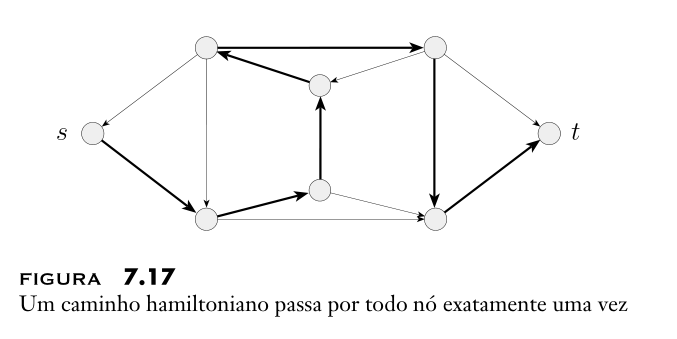
\includegraphics[width=9cm]{images/camHam.png}
		\end{center}
	\end{frame}	
	
	\begin{frame}[shrink]{Classe NP}
		\begin{block}{Característica importante}
			O problema $CAMHAM$ tem {\bf verificabilidade polinomial}
		\end{block} \pause
		\begin{block}{Outro problema polinomialmente verificável...}
			$COMPOSTOS = \{ x$ | $x = pq$, para inteiros $p,q > 1 \}$
		\end{block} \pause
		\begin{exampleblock}{Exemplo}
			$33 \in COMPOSTOS$ $\therefore$ \pause
			\begin{itemize}
				\item $3 \times 11 = 33$
				\item $3, 11 \in \mathbb{Z}$
			\end{itemize}
		\end{exampleblock} \pause
		\begin{alertblock}{Porém...}
			Existem problemas que não podem ser verificados em tempo polinomial. Exemplo: $\overline{CAMHAM}$.
		\end{alertblock}
	\end{frame}
	
	\begin{frame}{Classe NP}
		\begin{block}{Definição 7.18}
			Um {\bf verificador} para uma linguagem $A$ é um algoritmo $V$, em que
			\begin{center}
				$A = \{ \omega$ | $V$ aceita $\langle \omega, c \rangle$ para alguma cadeia $c \}$.
			\end{center}
		\end{block} \pause
		\begin{block}{Detalhes}
			Medimos o tempo de um verificador somente em termos do comprimento de $\omega$, portanto um {\bf verificador de tempo polinomial} roda em tempo polinomial no comprimento de $\omega$. 
		\end{block} \pause
		\begin{block}{Nomenclaturas...}
			Uma linguagem $A$ é {\bf polinomialmente verificável} se ela tem um verificador de tempo polinomial.
		\end{block}
	\end{frame}		
	
	\begin{frame}{Classe NP}
		\begin{block}{Certificado (Prova)}
			\begin{itemize}
				\item A informação adicional, representada por $c$, utilizada por um verificador é chamada de {\bf certificado} (ou prova) da pertinência a uma dada linguagem. \pause
				\item Para verificadores polinomiais, o certificado tem comprimento polinomial (no comprimento de $\omega$.
			\end{itemize}
		\end{block} \pause
		\begin{block}{Exemplo}
			\begin{itemize}
				\item Um certificado para uma cadeia $\langle G, s, t \rangle \in CAMHAM$ é um caminho hamiltoniano de $s$ a $t$. \pause
				\item Um certificado para um número composto $x \in COMPOSTOS $ é um dos seus divisores.
			\end{itemize}
		\end{block}
	\end{frame}
	
	\begin{frame}[shrink]{Classe NP}
		\begin{block}{Definição 7.19}
			{\bf NP} é a classe das linguagens que têm verificadores de tempo polinomial.
		\end{block} \pause
		\begin{block}{Teorema 7.20}
			Uma linguagem está em {\bf NP} sse ela é decidida por alguma máquina de Turing não-determinística de tempo polinomial.
		\end{block} \pause
		\begin{block}{Definição 7.21}
			{\bf NTIME(t(n))} = $\{L$ | $L$ é uma linguagem decidida por uma MT não-determinística de tempo $O(t(n)) \}$.
		\end{block} \pause
		\begin{exampleblock}{Corolário}
			{\bf NP} $ \cong \bigcup_k$ {\bf NTIME($n^k$)}
		\end{exampleblock}
	\end{frame}
	
	\begin{frame}{Classe NP}
		\begin{center}
			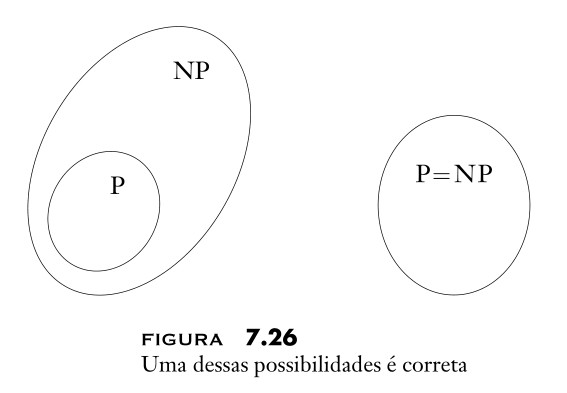
\includegraphics[width=9cm]{images/pNp.png}
		\end{center}
	\end{frame}		
	
	
	\begin{frame}
		\titlepage
	\end{frame}
	
\end{document}